\section{Measurement Scenario: Otaniemi Campus (Small Scene)}
\label{sec:otaniemi}

Otaniemi is an urban campus district located in Espoo, Finland, and home to
Aalto University's School of Electrical Engineering.
The broader campus area spans approximately $790\,\text{m}\times 645\,\text{m}$
and is characterised by a heterogeneous mix of mid-rise university buildings,
research laboratories, and student facilities, the majority of which are
constructed from reinforced concrete with glass
facades~\cite{itu_p2040}.
The irregular building layout creates a suburban micro-cell propagation
environment that combines open plazas with densely built corridors, producing
a channel that exhibits both strong line-of-sight (LOS) components across open
areas and rich non-line-of-sight (NLOS) multipath contributions from building
facades and corners~\cite{rappaport2013millimeter}.

For this project, a cropped sub-region of the full Otaniemi model is used
(henceforth the \emph{Otaniemi\_small} scene), covering
$x\in[-47.5,\,85.0]\,\text{m}$ and $y\in[-60.0,\,85.0]\,\text{m}$ around the
School of Electrical Engineering cluster.
This sub-region retains enough geometric diversity to challenge the
propagation and learning pipeline while keeping the total ray-tracing workload
tractable on a CPU-only host~\cite{hoydis2023sionna_rt,jakob2022mitsuba3}.

\subsection{Scene Geometry}

The three-dimensional scene is constructed from OpenStreetMap building
footprint data. Each polygon is extruded to a height derived from OSM
\texttt{height} or \texttt{building:levels} tags (assuming $3\,\text{m}$ per
storey, default $8\,\text{m}$). The coordinate origin is placed at the
bounding-box centroid, with the $+x$ axis pointing east and $+y$ pointing
north. Roof and wall meshes are triangulated to handle concave polygons, and
a flat ground plane covering the full scene extent is included as an
additional reflector.

\subsection{Base-Station and UE Layout}
\label{sec:scene_layout}

Rather than a single rooftop cell, the scene is instrumented with
\textbf{nine} rooftop base stations (TX0--TX8) at $z=19\,\text{m}$, whose
footprints are listed in Table~\ref{tab:tx_positions} and depicted in
Fig.~\ref{fig:scene_nodes}.
This multi-site layout produces distinguishable CSI fingerprints across
the scene and provides the spatial diversity required by both localization
and channel-charting algorithms~\cite{3gpp_nr_channel}.

UEs are sampled on a regular horizontal grid at pedestrian height
$z=1.25\,\text{m}$, with a lateral spacing of $2.5\,\text{m}$ across the
extents given above.
Grid points that fall inside a building footprint are pruned before ray
tracing, yielding \textbf{3\,186} valid UE positions which form the
fingerprint database used throughout
Sections~\ref{sec:localization}--\ref{sec:channel_charting}.
A sample density of a few points per $\text{m}^2$ is consistent with the
course guideline that supports localization accuracy on the order of
$1\,\text{m}$ under ideal propagation conditions.

\begin{table}[htbp]
  \caption{Base-station coordinates (metres), all at $z=19\,\text{m}$}
  \label{tab:tx_positions}
  \centering
  \begin{tabular}{lrr}
    \toprule
    Site & $x$ (m) & $y$ (m) \\
    \midrule
    TX0 & $-5.0$  & $70.0$  \\
    TX1 & $-33.0$ & $-17.0$ \\
    TX2 & $-3.0$  & $14.0$  \\
    TX3 & $-6.0$  & $-40.0$ \\
    TX4 & $55.0$  & $-52.5$ \\
    TX5 & $61.0$  & $7.0$   \\
    TX6 & $49.0$  & $46.0$  \\
    TX7 & $28.0$  & $-41.0$ \\
    TX8 & $84.0$  & $-18.0$ \\
    \bottomrule
  \end{tabular}
\end{table}

\begin{figure}[htbp]
  \centering
  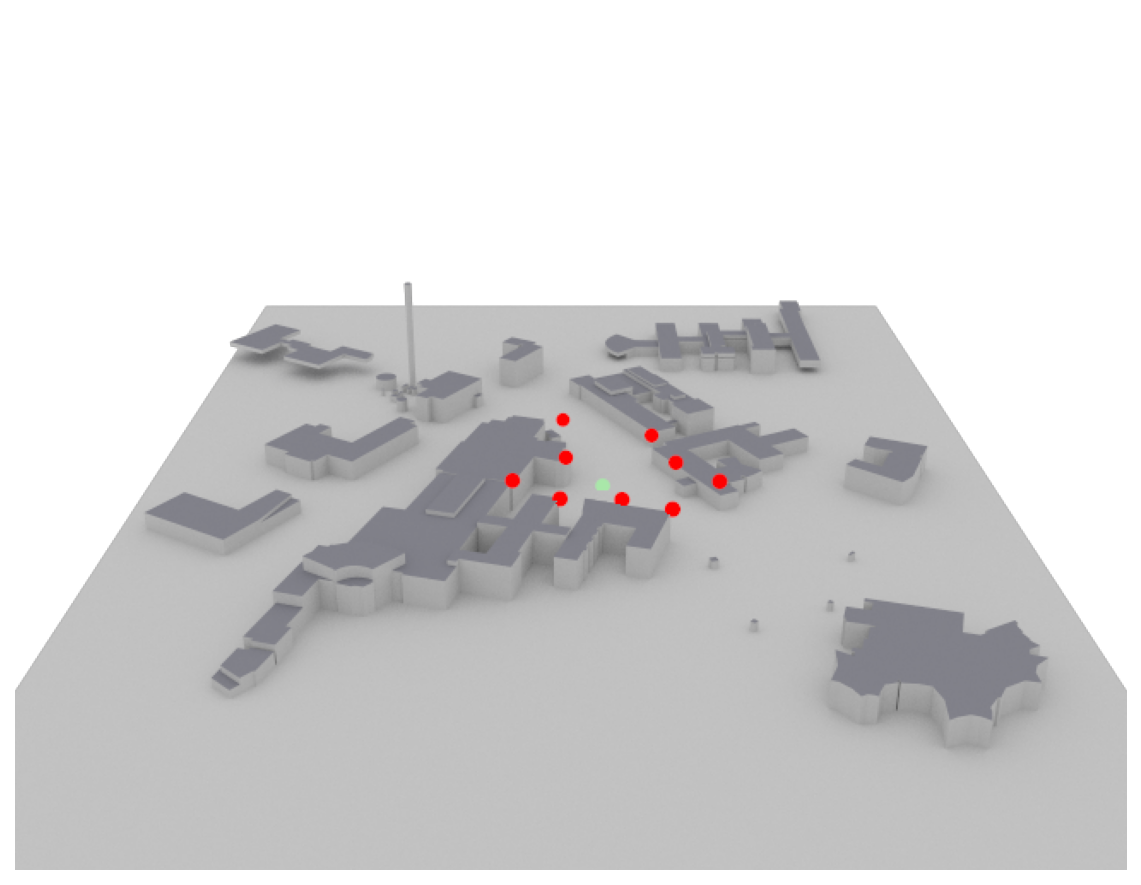
\includegraphics[width=\columnwidth]{pictures/01_generate_dataset/scene_with_devices.png}
  \caption{Otaniemi\_small scene with the nine rooftop base stations and
           the reference UE indicated. UEs are sampled on a $2.5\,$m grid
           across the scene extents.}
  \label{fig:scene_nodes}
\end{figure}


\subsection{Electromagnetic Material Properties}

Surface materials are assigned from OSM \texttt{building:material} tags
and follow ITU-R~P.2040-3~\cite{itu_p2040}; parameters at $3.6\,\text{GHz}$
are listed in Table~\ref{tab:materials}.
Concrete is the dominant wall material and produces strong near-specular
reflections.
Glass facades, present on several modern campus buildings, introduce partial
transmission and weaker reflections.
The ground plane is assigned a medium dry-ground model, representative of
typical soil and paved surfaces at the site.

\begin{table}[htbp]
  \caption{ITU-R P.2040-3 material parameters at $f_c = 3.6\,\text{GHz}$}
  \label{tab:materials}
  \centering
  \begin{tabular}{llrr}
    \toprule
    Surface & Sionna ID & $\varepsilon_r$ & $\sigma$ (S/m) \\
    \midrule
    Building walls (default) & \texttt{itu\_concrete}          & 5.31 & 0.090 \\
    Glass facades            & \texttt{itu\_glass}             & 6.27 & 0.000 \\
    Metal cladding           & \texttt{itu\_metal}             & ---  & $\to\infty$ \\
    Ground plane             & \texttt{itu\_medium\_dry\_ground} & 15.0 & 0.035 \\
    \bottomrule
  \end{tabular}
\end{table}
